\documentclass[]{article}
\usepackage{stata}
\usepackage{lmodern}
\usepackage{amssymb,amsmath}
\usepackage{ifxetex,ifluatex}
\usepackage{fixltx2e} % provides \textsubscript
\ifnum 0\ifxetex 1\fi\ifluatex 1\fi=0 % if pdftex
  \usepackage[T1]{fontenc}
  \usepackage[utf8]{inputenc}
\else % if luatex or xelatex
  \ifxetex
    \usepackage{mathspec}
  \else
    \usepackage{fontspec}
  \fi
  \defaultfontfeatures{Ligatures=TeX,Scale=MatchLowercase}
\fi
% use upquote if available, for straight quotes in verbatim environments
\IfFileExists{upquote.sty}{\usepackage{upquote}}{}
% use microtype if available
\IfFileExists{microtype.sty}{%
\usepackage[]{microtype}
\UseMicrotypeSet[protrusion]{basicmath} % disable protrusion for tt fonts
}{}
\PassOptionsToPackage{hyphens}{url} % url is loaded by hyperref
\usepackage[unicode=true]{hyperref}
\hypersetup{
            pdftitle={API 201Z Stata Demonstration},
            pdfauthor={Shiro Kuriwaki},
            pdfborder={0 0 0},
            breaklinks=true}
\urlstyle{same}  % don't use monospace font for urls
\usepackage{graphicx,grffile}
\makeatletter
\def\maxwidth{\ifdim\Gin@nat@width>\linewidth\linewidth\else\Gin@nat@width\fi}
\def\maxheight{\ifdim\Gin@nat@height>\textheight\textheight\else\Gin@nat@height\fi}
\makeatother
% Scale images if necessary, so that they will not overflow the page
% margins by default, and it is still possible to overwrite the defaults
% using explicit options in \includegraphics[width, height, ...]{}
\setkeys{Gin}{width=\maxwidth,height=\maxheight,keepaspectratio}
\IfFileExists{parskip.sty}{%
\usepackage{parskip}
}{% else
\setlength{\parindent}{0pt}
\setlength{\parskip}{6pt plus 2pt minus 1pt}
}
\setlength{\emergencystretch}{3em}  % prevent overfull lines
\providecommand{\tightlist}{%
  \setlength{\itemsep}{0pt}\setlength{\parskip}{0pt}}
\setcounter{secnumdepth}{0}
% Redefines (sub)paragraphs to behave more like sections
\ifx\paragraph\undefined\else
\let\oldparagraph\paragraph
\renewcommand{\paragraph}[1]{\oldparagraph{#1}\mbox{}}
\fi
\ifx\subparagraph\undefined\else
\let\oldsubparagraph\subparagraph
\renewcommand{\subparagraph}[1]{\oldsubparagraph{#1}\mbox{}}
\fi

% set default figure placement to htbp
\makeatletter
\def\fps@figure{htbp}
\makeatother


\title{API 201Z Stata Demonstration}
\author{Shiro Kuriwaki}
\date{September 6th, 2018}

\begin{document}
\maketitle

\section{Scripts and Console}\label{scripts-and-console}

How does one ``do Stata''? We interact with Stata by sending the
statistical program ``commands''. Commands can be anything from reading
in a dataset to running a regression.

\begin{figure}
\centering
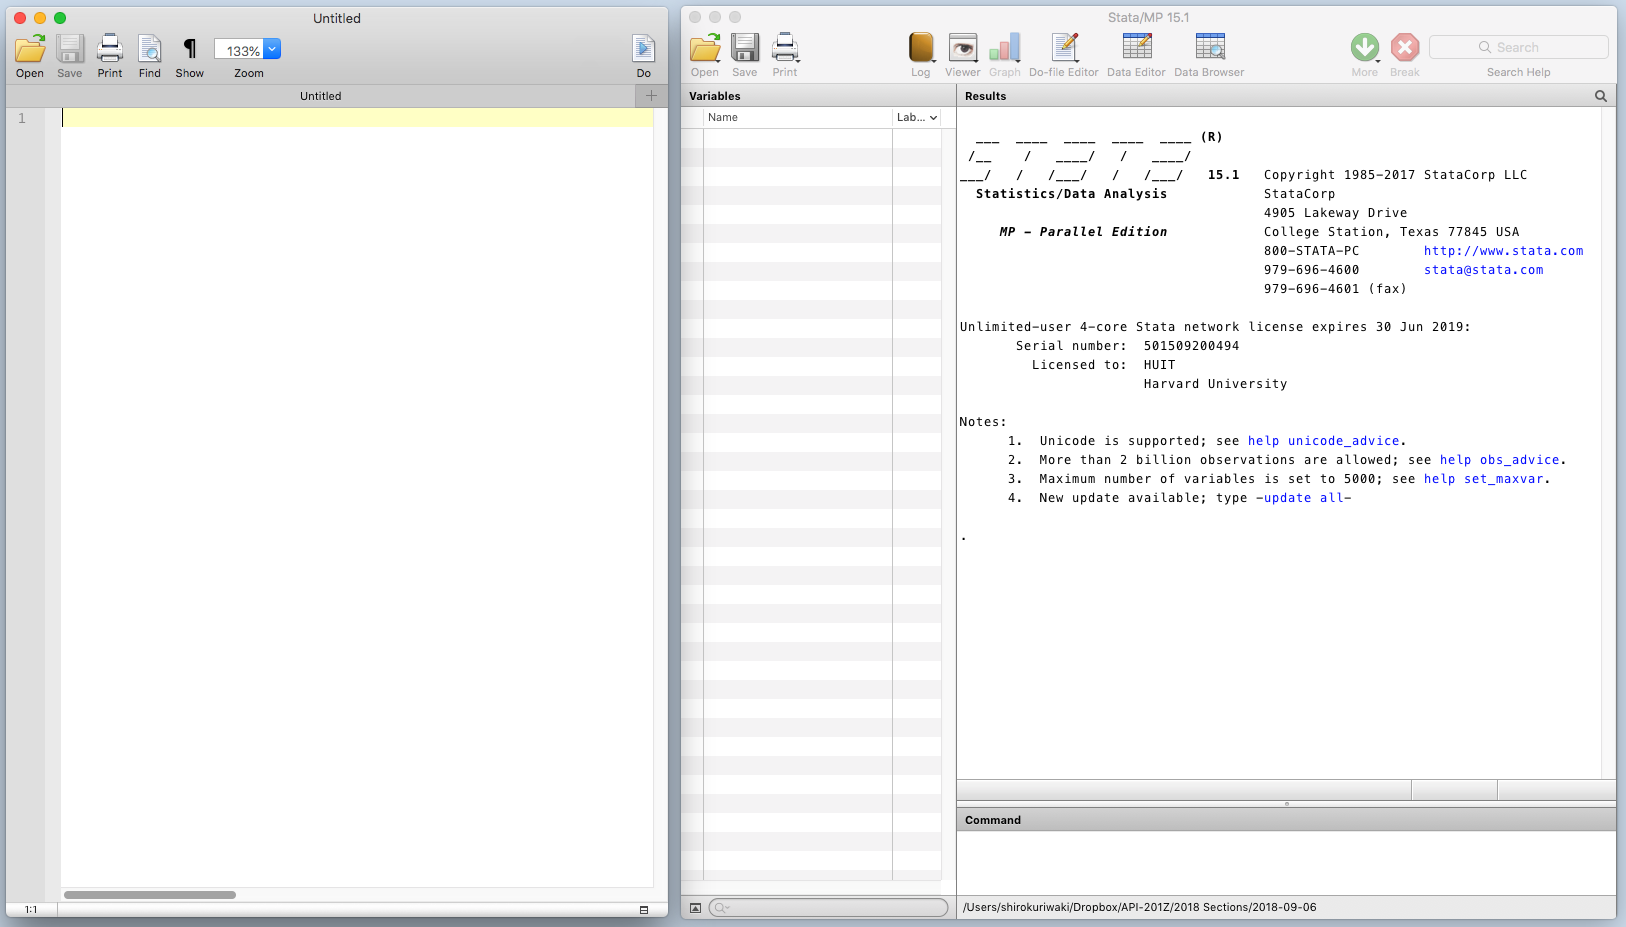
\includegraphics[width=0.90000\textwidth]{statawindow.png}
\caption{What's what in a Stata Window}
\end{figure}

\section{Starting Fresh}\label{starting-fresh}

Stata takes one dataset at a time and runs manipulations on it. To clear
the memory (i.e.~the dataset and other auxilarly objects) in Stata, the
command is:

\begin{stlog}
. clear all
{\smallskip}
\end{stlog}

For the above code and all other Stata code in this document, you can
run it after removing the period \texttt{.} in the beginning -- which
indicates a command that was already entered.

\section{Getting Help}\label{getting-help}

If you know the name of the function you want to use but aren't sure how
to use it, use the help command by typing in \texttt{help} and then the
name of the function.

\begin{stlog}
. help ivregress
{\smallskip}
\end{stlog}

If you do not know the exact name of the function, you can Google or
search on Stata's help manual / search box.

\section{Logging your Activity}\label{logging-your-activity}

Stata commands are stored in a script. You \emph{can} write commands
directly into the command window to get similar results. However, it is
often a bad idea to do your analysis through the command window because
it is easy to forget the exact steps. Instead, you should save your
commands in a script -- a \texttt{.do} file. When we ask for scripts on
problem sets, we are looking for a script.

The \texttt{.do} file lacks a way to store the output of your commands.
To store output you can generate a separate log file along with your
\texttt{.do} scripts. To do so,

start your \texttt{.do} file with

\begin{verbatim}
log using kuriwaki_log.txt, text replace
\end{verbatim}

where the filename \texttt{kuriwaki\_log.txt} can be replaced by any
name of your choice.

Then at the end of your \texttt{.do} file, enter

\begin{verbatim}
log close
\end{verbatim}

to close the log.

Finally, you also might want to enter at the very first line, before
\texttt{log\ using...}, the following

\begin{verbatim}
capture log close
\end{verbatim}

to close any already opened logs (if they exist).

\section{Reading in Data}\label{reading-in-data}

When working in Stata, it's always an important first step to make sure
you're in the right working directory (where you tell Stata what folder
you want to work in).

\texttt{pwd} stands for ``present working directory''. \texttt{cd}
stands for ``change directory''. \texttt{ls} stands for ``list (the
files in current directory)''. \texttt{.} is shorthand for the current
directory, \texttt{..} for the parent directory, and
\texttt{\textasciitilde{}/} for your home directory.

For example,

\begin{verbatim}
cd "~/Dropbox/temp"
\end{verbatim}

You will want to modify the path above to your own.

Now, load the \texttt{.dta} file provided into Stata:

\begin{stlog}
. use sample_data.dta
{\smallskip}
\end{stlog}

Note that \texttt{use} is limited to \texttt{.dta} files; Stata's
designated way of storing datasets. The most useful feature of a
\texttt{.dta} format is that the data values comes with \texttt{labels}.
For example, a \texttt{.dta} will be able to store the fact that the
labels \texttt{female} and \texttt{male} correspond to values 1 and 2,
respectively.

Sometimes, your data will not come in a \texttt{.dta} format. A basic
format is \texttt{.csv} -- standing for comma-separated-values. These
files is like an Excel spreadsheet, but without any of the formatting
(color, functions, comments). The csv is a common and desirable form in
programming, as it can be read by any statistical program.

What if we needed to load a csv file?

\begin{stlog}
. import delimited using sample_data.csv, clear
(7 vars, 435 obs)
{\smallskip}
\end{stlog}

We see that compared to the one-word \texttt{use}, the Stata syntax is a
bit more lengthy to read in a spreadsheet. Again, enter
\texttt{help\ import} or \texttt{help\ import\ delimited} to understand
thi son your own. The help page tells us that we use
\texttt{import\ delimited} and then the file name followed by the
\texttt{using} word.

\section{A comma separates commands and
options}\label{a-comma-separates-commands-and-options}

You will see the comma used many times in Stata code. On the left-side
of the comma, you put the main command. On the right-side, you put
secondary options. The comma often confuses first-time users.

\begin{stlog}
. clear all
{\smallskip}
\end{stlog}

\section{Built-in Data}\label{built-in-data}

To go through how to analyze and review data, let's work with a dataset
that is pre-loaded into the Stata app.

The command \texttt{sysuse} is a command to use a data already baked
into the system. Then \texttt{nlsw88} is one of the several datasets
that are available.

This is an extract from the 1988 National Longitudinal Survey of Women,
which is a survey conducted by the Department of Labor. This extract
contains about 2000 women in their 30s and 40s.

\begin{stlog}
. sysuse nlsw88
(NLSW, 1988 extract)
{\smallskip}
\end{stlog}

\section{Browsing Data}\label{browsing-data}

To look at the data we've just loaded in, use the command
\texttt{browse} (or \texttt{br} for short):

\begin{verbatim}
browse
\end{verbatim}

To get a list of the variables and the variable types:

\begin{stlog}
. describe
{\smallskip}
Contains data from /Applications/Stata/ado/base/n/nlsw88.dta
  obs:         2,246                          NLSW, 1988 extract
 vars:            17                          1 May 2016 22:52
 size:        60,642                          (_dta has notes)
\HLI{79}
              storage   display    value
variable name   type    format     label      variable label
\HLI{79}
idcode          int     \%8.0g                 NLS id
age             byte    \%8.0g                 age in current year
race            byte    \%8.0g      racelbl    race
married         byte    \%8.0g      marlbl     married
never_married   byte    \%8.0g                 never married
grade           byte    \%8.0g                 current grade completed
collgrad        byte    \%16.0g     gradlbl    college graduate
south           byte    \%8.0g                 lives in south
smsa            byte    \%9.0g      smsalbl    lives in SMSA
c_city          byte    \%8.0g                 lives in central city
industry        byte    \%23.0g     indlbl     industry
occupation      byte    \%22.0g     occlbl     occupation
union           byte    \%8.0g      unionlbl   union worker
wage            float   \%9.0g                 hourly wage
hours           byte    \%8.0g                 usual hours worked
ttl_exp         float   \%9.0g                 total work experience
tenure          float   \%9.0g                 job tenure (years)
\HLI{79}
Sorted by: idcode
{\smallskip}
\end{stlog}

\section{Summary Statistics}\label{summary-statistics}

We can see that there are seventeen variables in this dataset.

\begin{stlog}
. sum age
{\smallskip}
    Variable {\VBAR}        Obs        Mean    Std. Dev.       Min        Max
\HLI{13}{\PLUS}\HLI{57}
         age {\VBAR}      2,246    39.15316    3.060002         34         46
{\smallskip}
\end{stlog}

\begin{stlog}
. sum age, detail
{\smallskip}
                     age in current year
\HLI{61}
      Percentiles      Smallest
 1\%           34             34
 5\%           35             34
10\%           35             34       Obs               2,246
25\%           36             34       Sum of Wgt.       2,246
{\smallskip}
50\%           39                      Mean           39.15316
                        Largest       Std. Dev.      3.060002
75\%           42             45
90\%           44             45       Variance       9.363614
95\%           44             46       Skewness       .2003234
99\%           45             46       Kurtosis       1.932389
{\smallskip}
\end{stlog}

\begin{stlog}
. tabstat age, stat(mean sd median iqr)
{\smallskip}
    variable {\VBAR}      mean        sd       p50       iqr
\HLI{13}{\PLUS}\HLI{40}
         age {\VBAR}  39.15316  3.060002        39         6
\HLI{13}{\BOTT}\HLI{40}
{\smallskip}
\end{stlog}

\section{New Variables}\label{new-variables}

To create a new variable, use the \texttt{generate} (\texttt{gen} for
short) command:

\begin{stlog}
. gen weekly_wage = wage * hours
(4 missing values generated)
{\smallskip}
\end{stlog}

Stata, along with SPSS, adds ``labels'' to variables. You might think of
the labels as ``pretty names'' that are more legible than
``weekly\_wage''. labels show up in the Stata variable window and are
also get used in graphs. It is often worth the extra effort to label
your own variables.

\begin{stlog}
. label variable weekly_wage "weekly wage (estimate)"
{\smallskip}
\end{stlog}

If you want to redefine a variable, use the \texttt{replace} command:

\begin{stlog}
. gen foo = (age){\caret}2
{\smallskip}
. replace foo = 0
(2,246 real changes made)
{\smallskip}
\end{stlog}

To ``drop'' (delete) a variable:

\begin{stlog}
. drop foo
{\smallskip}
\end{stlog}

\section{Counting}\label{counting}

To count the rows in your dataset,

\begin{stlog}
. count
  2,246
{\smallskip}
\end{stlog}

What about counting only observations that match a certain condition?
Use \texttt{if} at the end and the boolean conditions \texttt{==},
\texttt{!=}, \texttt{\textbar{}}, and \texttt{\&}.

\begin{stlog}
. count if south == 1
  942
{\smallskip}
\end{stlog}

\texttt{tabulate} is an oft-used function for counting. We can either do
a one-way or two-way tabulation.

One-way tabs is a tabulation of counts

\begin{stlog}
. tabulate c_city
{\smallskip}
   lives in {\VBAR}
    central {\VBAR}
       city {\VBAR}      Freq.     Percent        Cum.
\HLI{12}{\PLUS}\HLI{35}
          0 {\VBAR}      1,591       70.84       70.84
          1 {\VBAR}        655       29.16      100.00
\HLI{12}{\PLUS}\HLI{35}
      Total {\VBAR}      2,246      100.00
{\smallskip}
\end{stlog}

Two-way tabs is referred to as a ``crosstab''

\begin{stlog}
. tabulate c_city union
{\smallskip}
  lives in {\VBAR}
   central {\VBAR}     union worker
      city {\VBAR}  nonunion      union {\VBAR}     Total
\HLI{11}{\PLUS}\HLI{22}{\PLUS}\HLI{10}
         0 {\VBAR}     1,034        288 {\VBAR}     1,322 
         1 {\VBAR}       383        173 {\VBAR}       556 
\HLI{11}{\PLUS}\HLI{22}{\PLUS}\HLI{10}
     Total {\VBAR}     1,417        461 {\VBAR}     1,878 
{\smallskip}
{\smallskip}
\end{stlog}

\section{Visualizing Data}\label{visualizing-data}

The \texttt{hist} command will generate a histogram.

\begin{stlog}
. hist wage
(bin=33, start=1.0049518, width=1.2042921)
{\smallskip}
. graph export hist_wage.png, width(2000) replace
(file hist_wage.png written in PNG format)
{\smallskip}
\end{stlog}

\begin{figure}
\centering
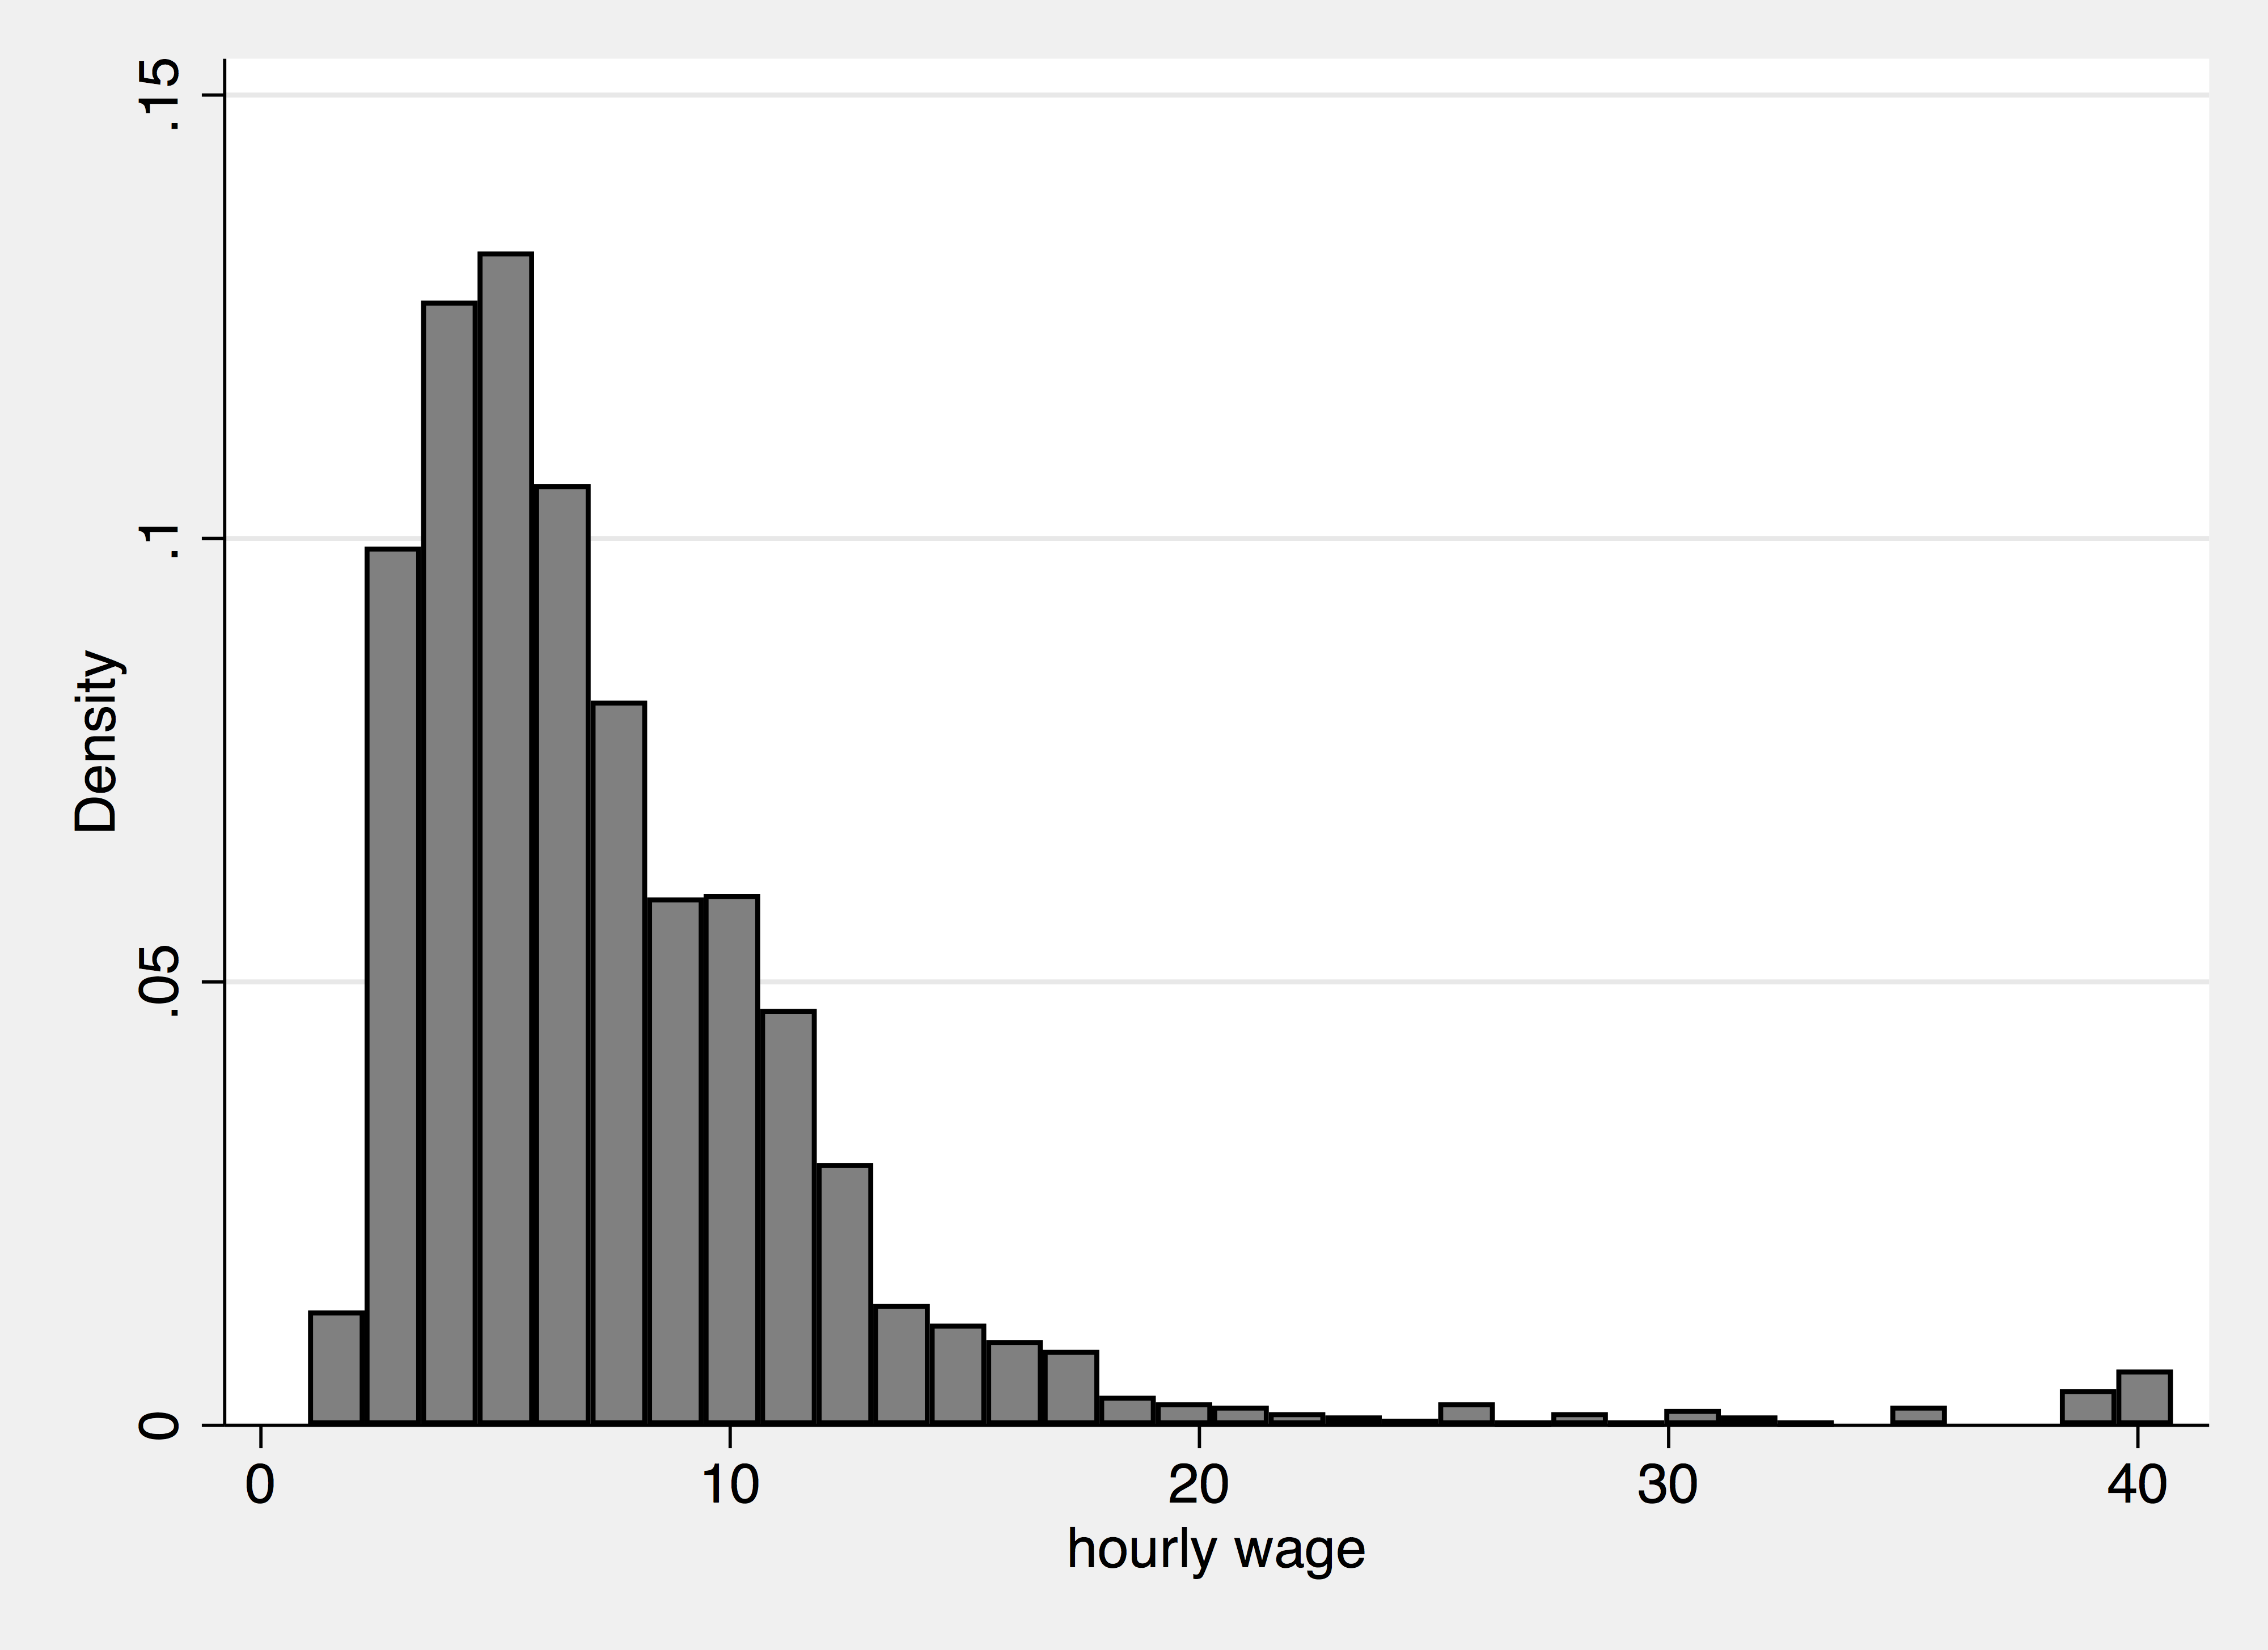
\includegraphics[width=1.00000\textwidth]{hist_wage.png}
\caption{}
\end{figure}

Note that we have two commands -- \texttt{hist} and
\texttt{graph\ export}. The first generates the figure within Stata; the
second saves that figure as a file on your computer. Saving files will
be make your workflow easier than saving files through the
click-and-drag interface each time.

The \texttt{scatter} command will generate a scatterplot. Two
variables\ldots{}two dimensions. The y-variable comes first, then the
x-variable:

\begin{stlog}
. scatter weekly_wage grade
{\smallskip}
. graph export edu_wage.png, width(1800) replace
(file edu_wage.png written in PNG format)
{\smallskip}
\end{stlog}

\begin{figure}
\centering
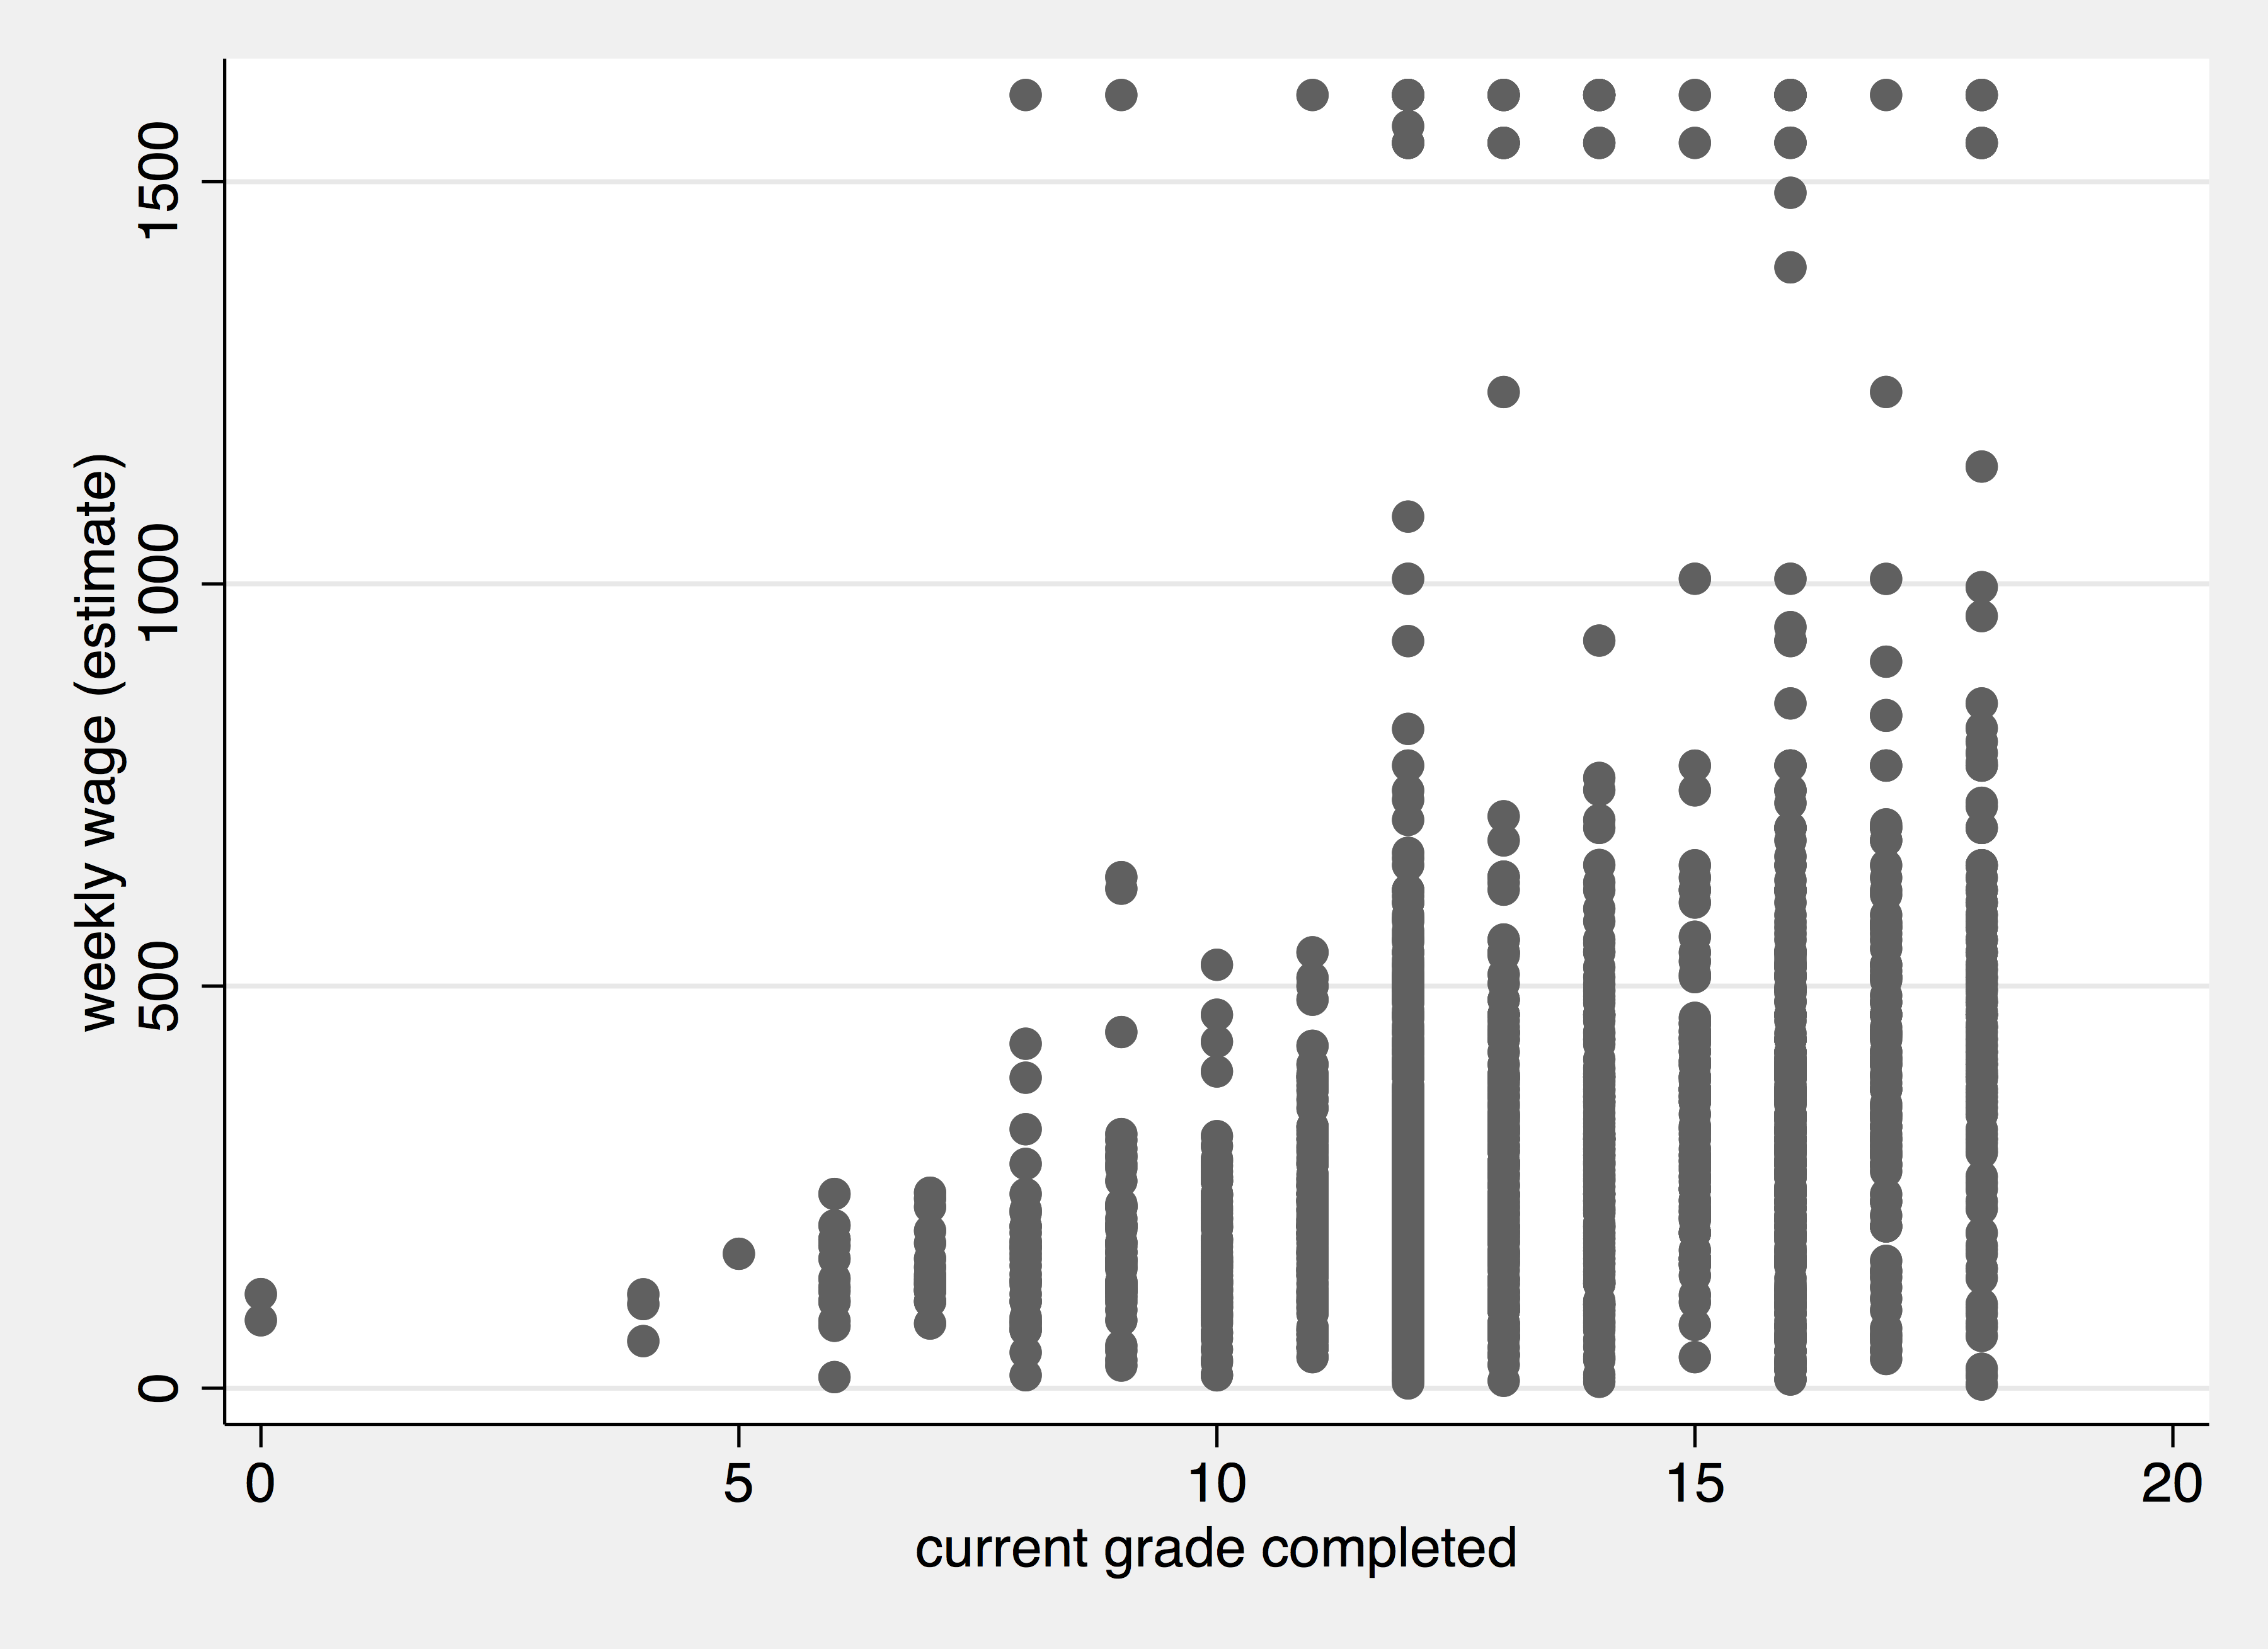
\includegraphics[width=1.00000\textwidth]{edu_wage.png}
\caption{}
\end{figure}

The \texttt{graph\ export} has many options beyond the default, and they
come after a comma \texttt{,}. Again, this is a general Stata rule --
options come after a comma. Like all commands, use the command
\texttt{help} (as in \texttt{help\ graph\ export}) to see all of them.

For example, we notice that the points above are overlapping and it is
hard to distinguish whether a point overlap with one other point or 100s
of other points. To this we could make the points transparent.

\begin{stlog}
. scatter weekly_wage grade, mcolor(\%30)
{\smallskip}
. graph export edu_wage_alpha.png, width(1800) replace
(file edu_wage_alpha.png written in PNG format)
{\smallskip}
\end{stlog}

\begin{figure}
\centering
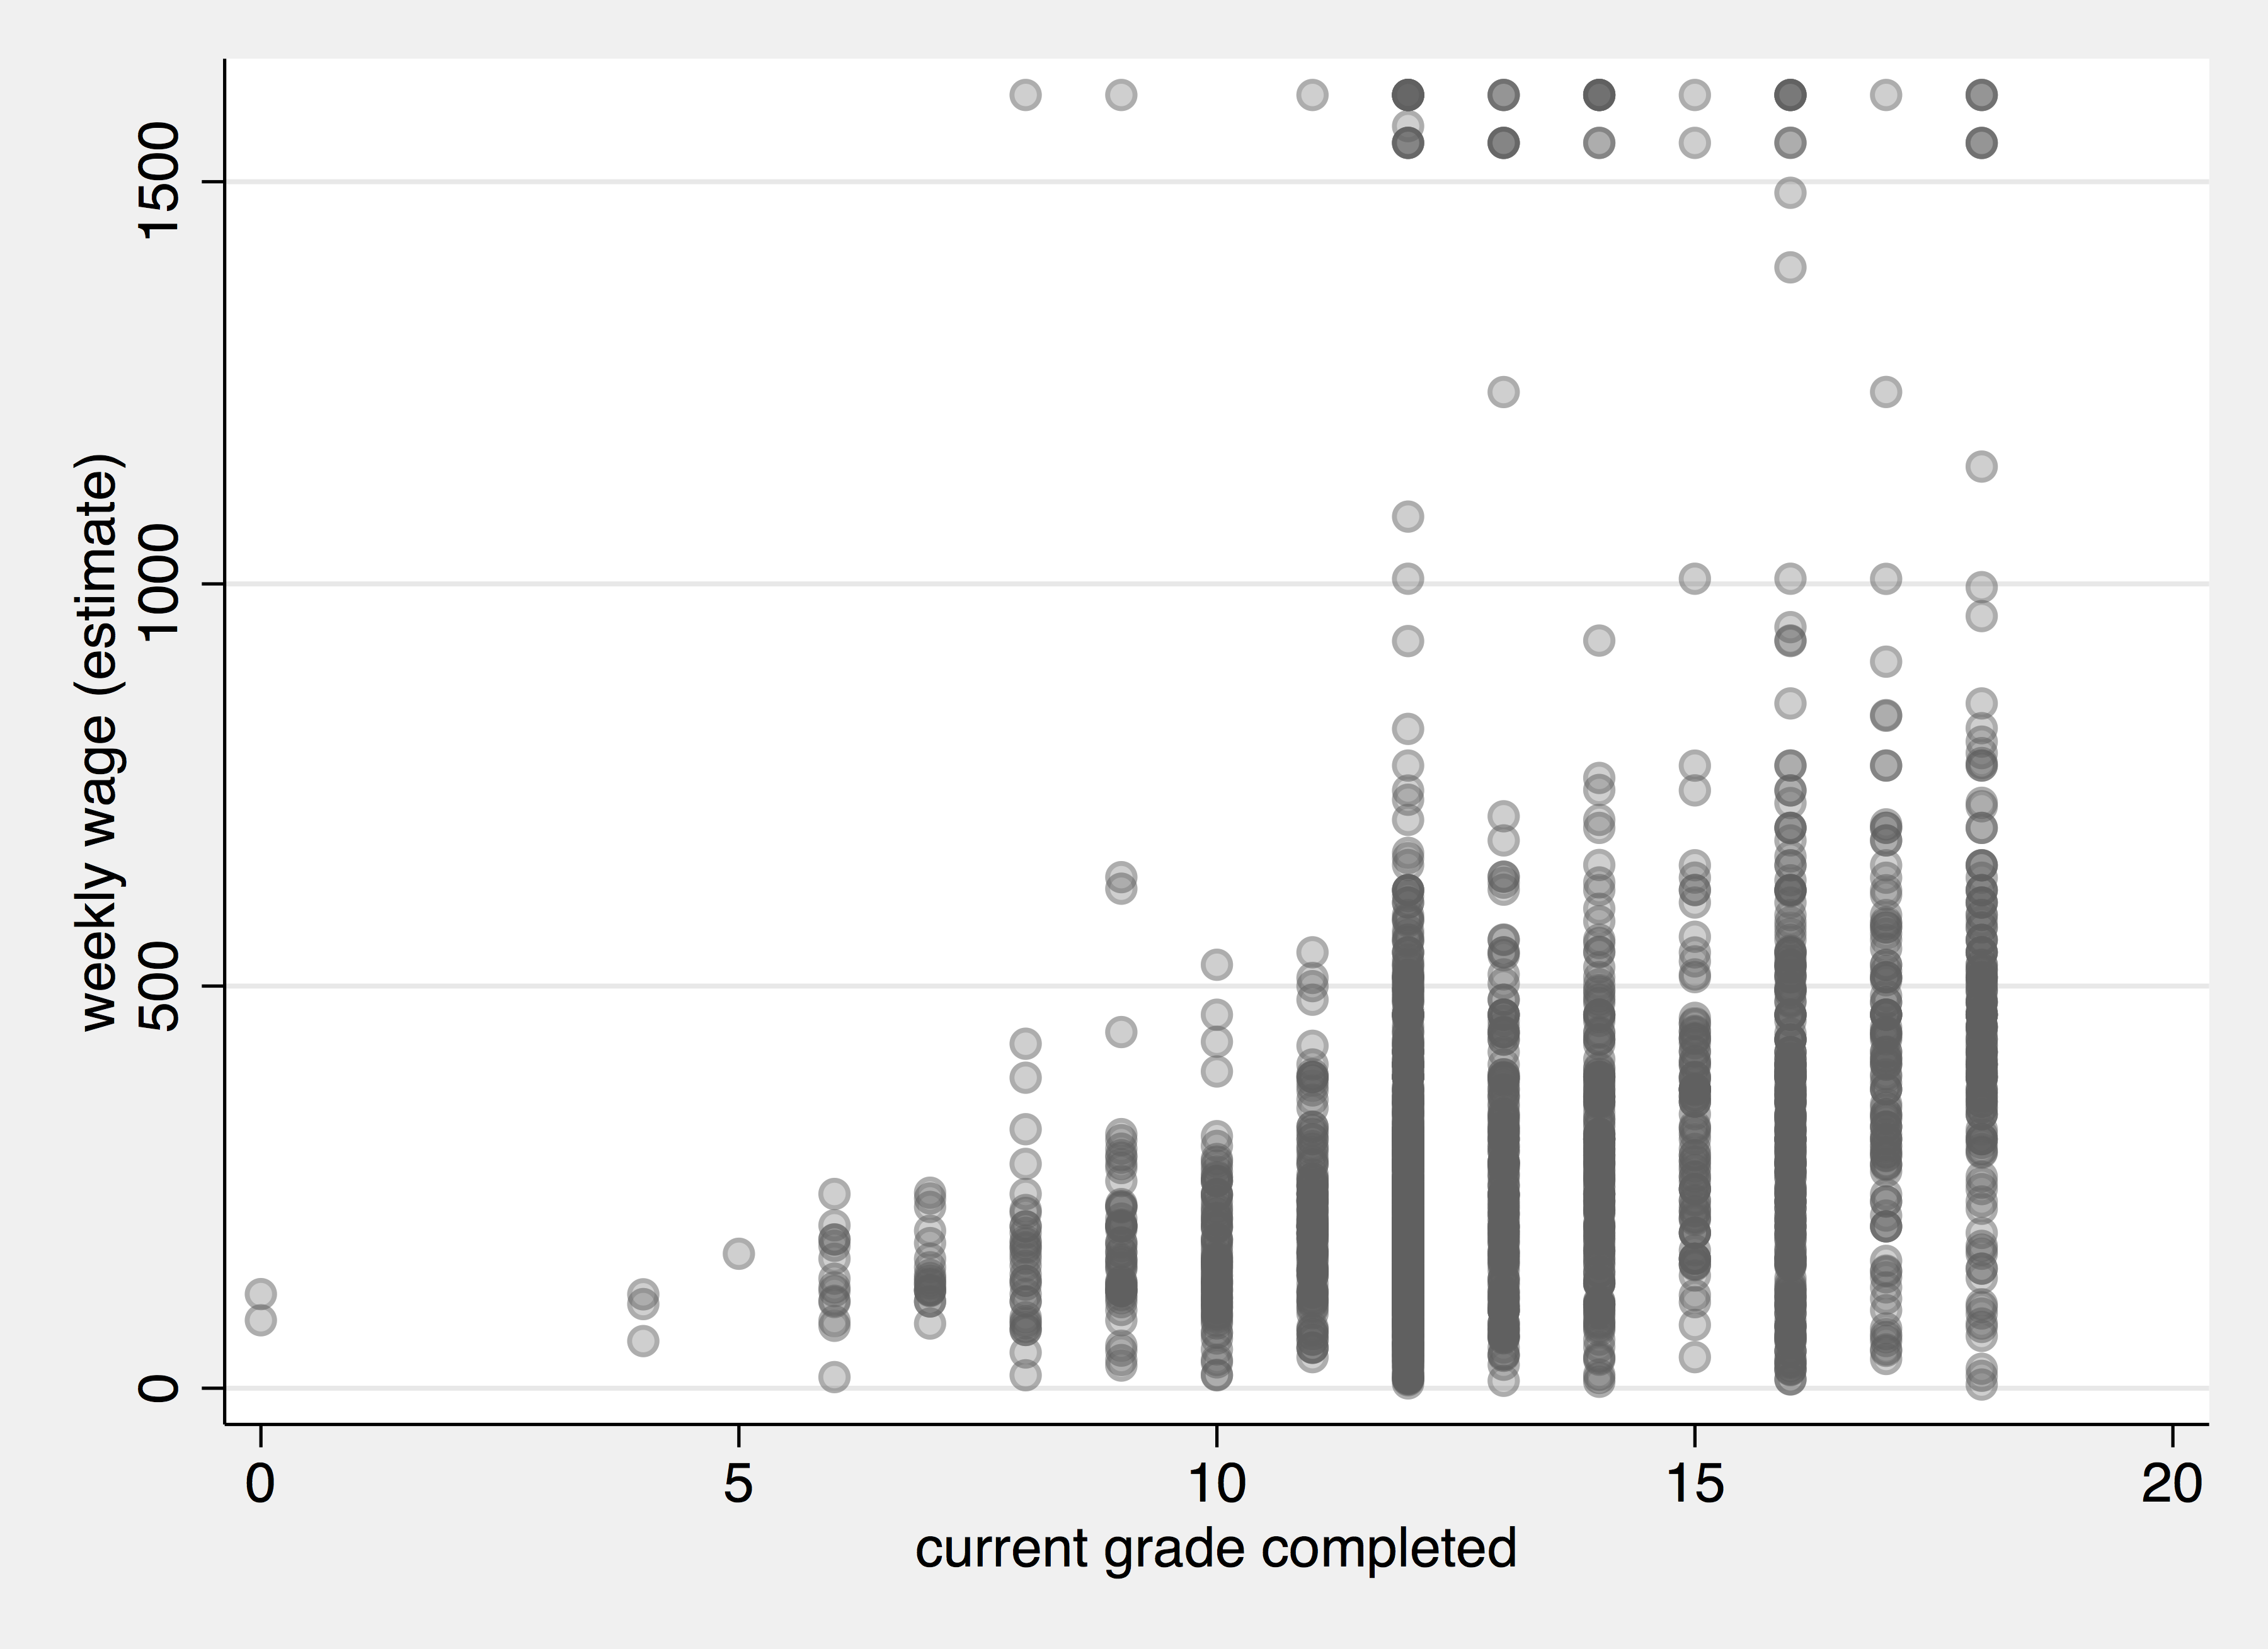
\includegraphics[width=1.00000\textwidth]{edu_wage_alpha.png}
\caption{}
\end{figure}

What if we only wanted to plot the wage of of blacks? We want to use a
conditional \texttt{"if"} statement:

\begin{stlog}
. hist wage if race == "black":racelbl
(bin=24, start=1.1513683, width=1.6498009)
{\smallskip}
. graph export wage_blk.png, width(2000) replace
(file wage_blk.png written in PNG format)
{\smallskip}
\end{stlog}

\begin{figure}
\centering
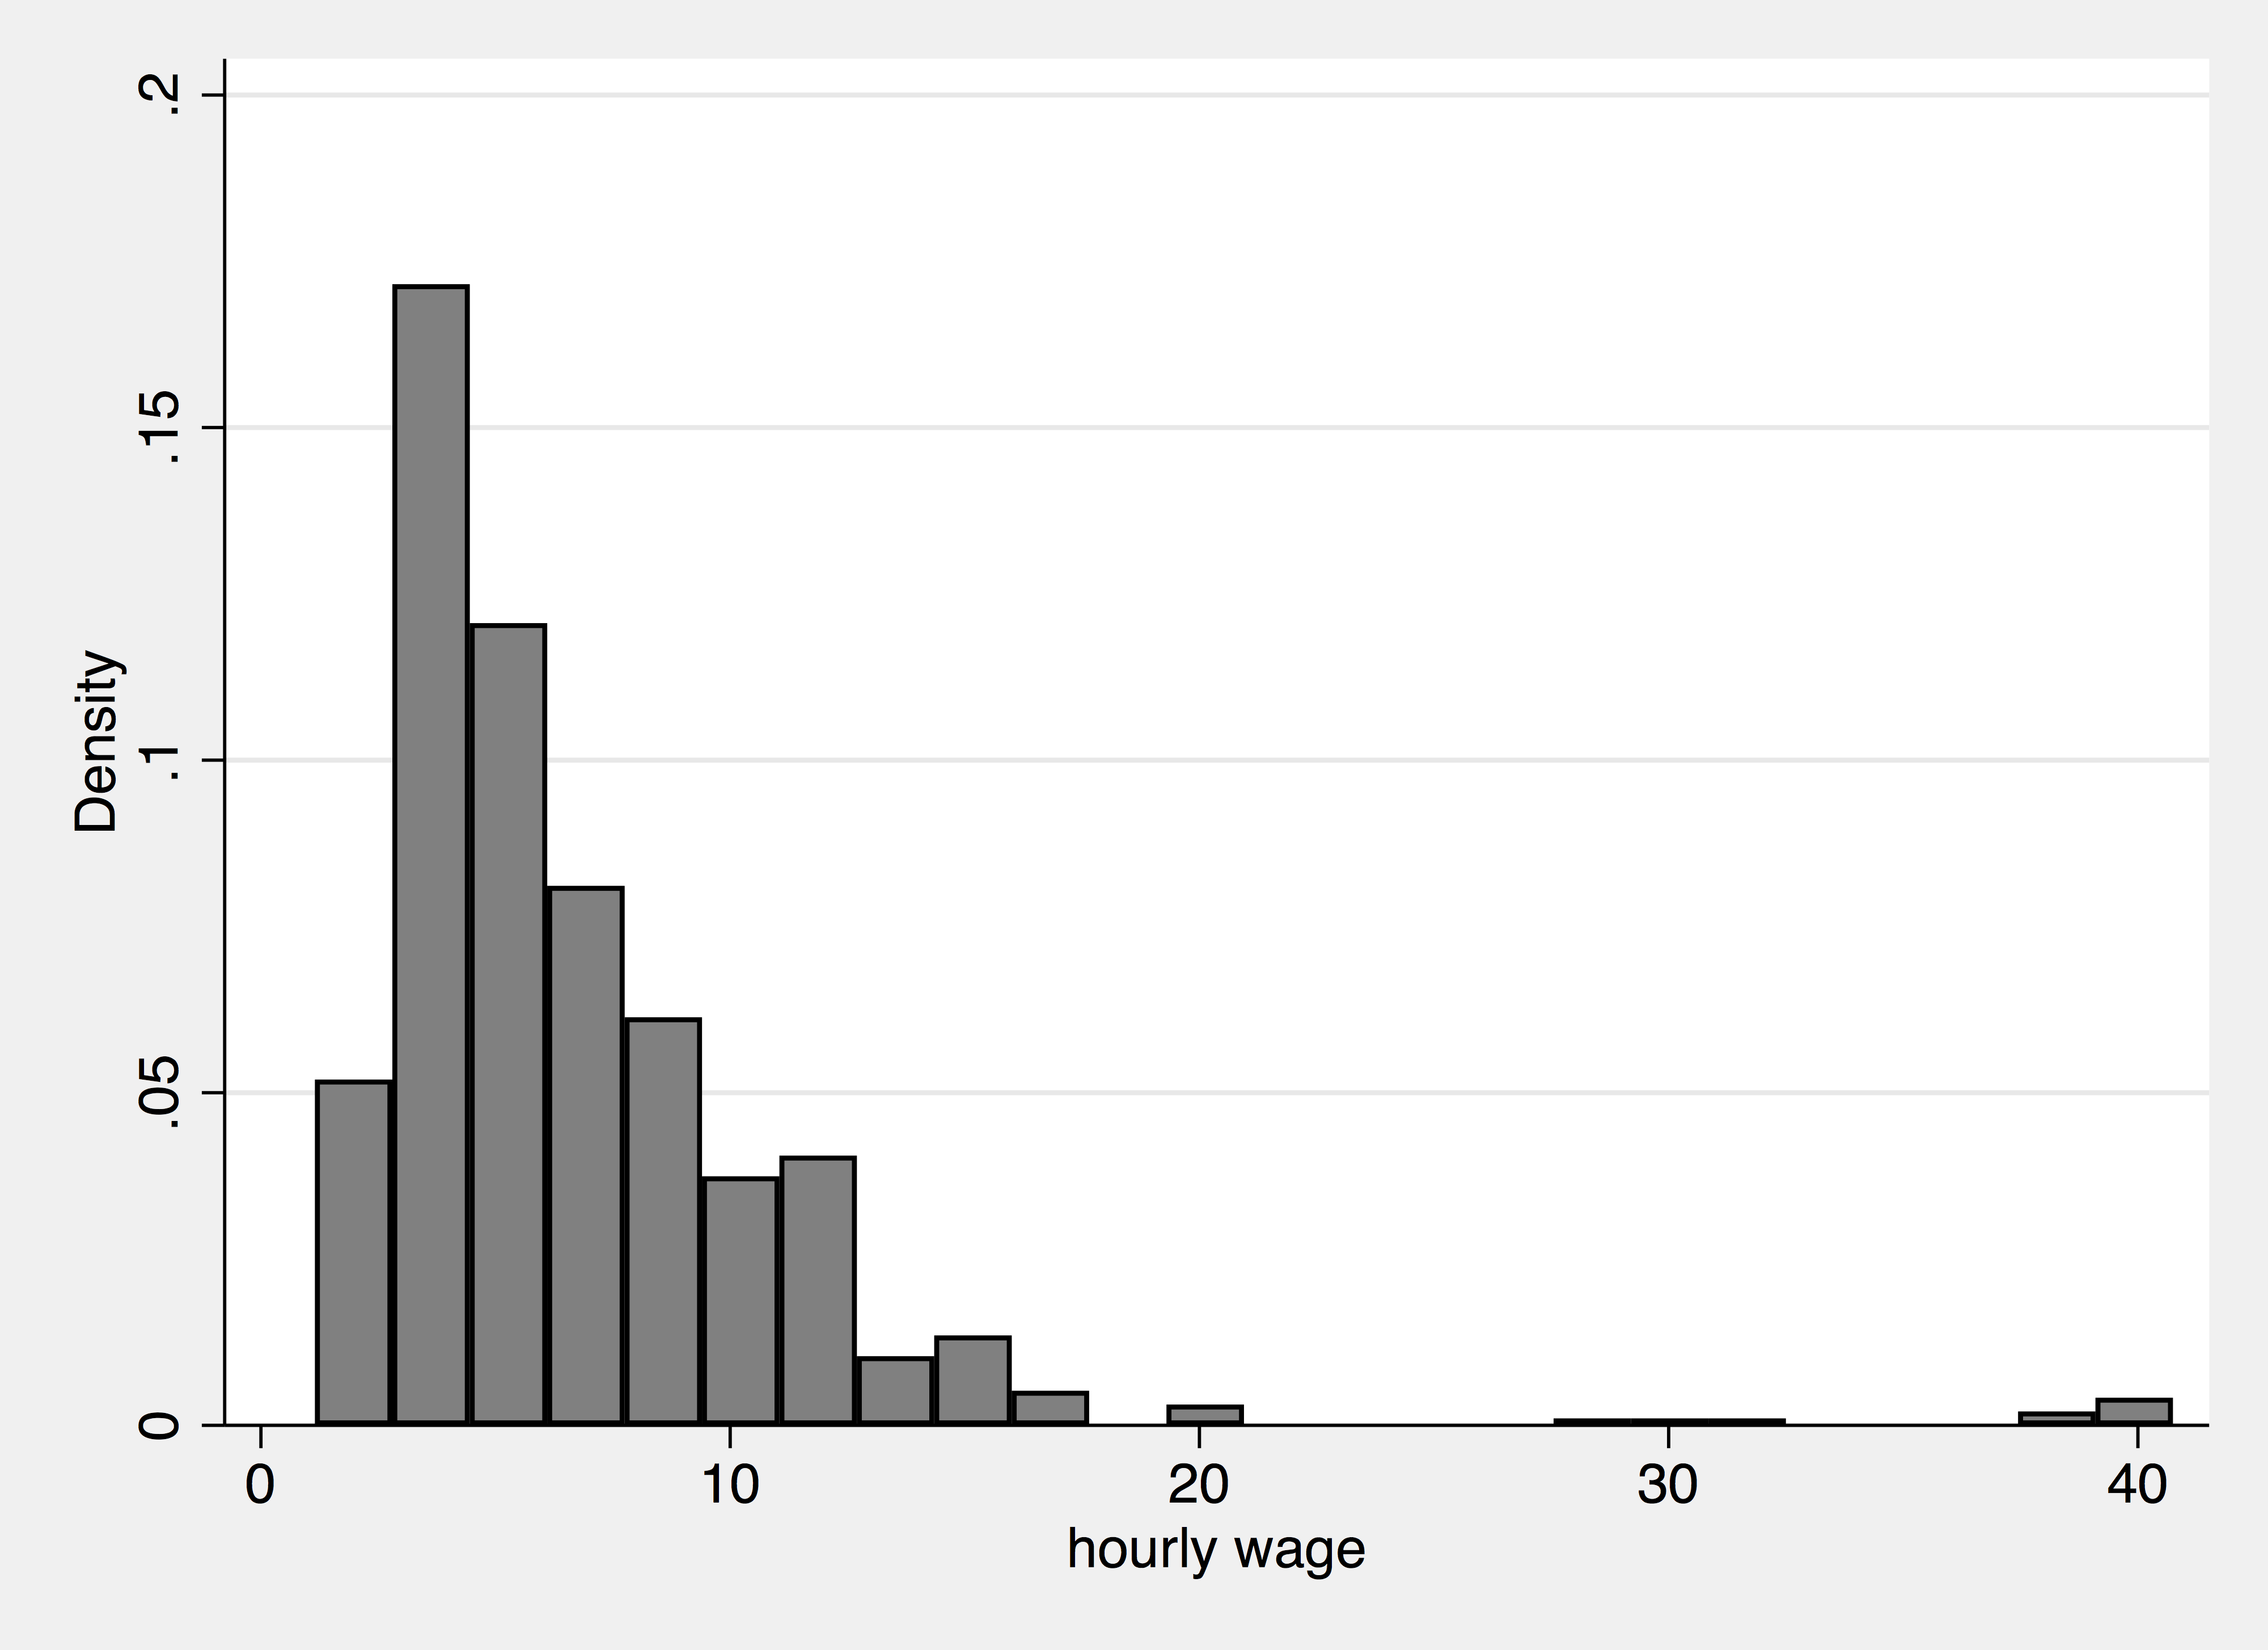
\includegraphics[width=1.00000\textwidth]{wage_blk.png}
\caption{}
\end{figure}

To compare the distribution of the same variable across groups, a
boxplot is useful

\begin{stlog}
. graph box wage, over(race)
{\smallskip}
. graph export race_wage.png, width(2000) replace
(file race_wage.png written in PNG format)
{\smallskip}
\end{stlog}

\begin{figure}
\centering
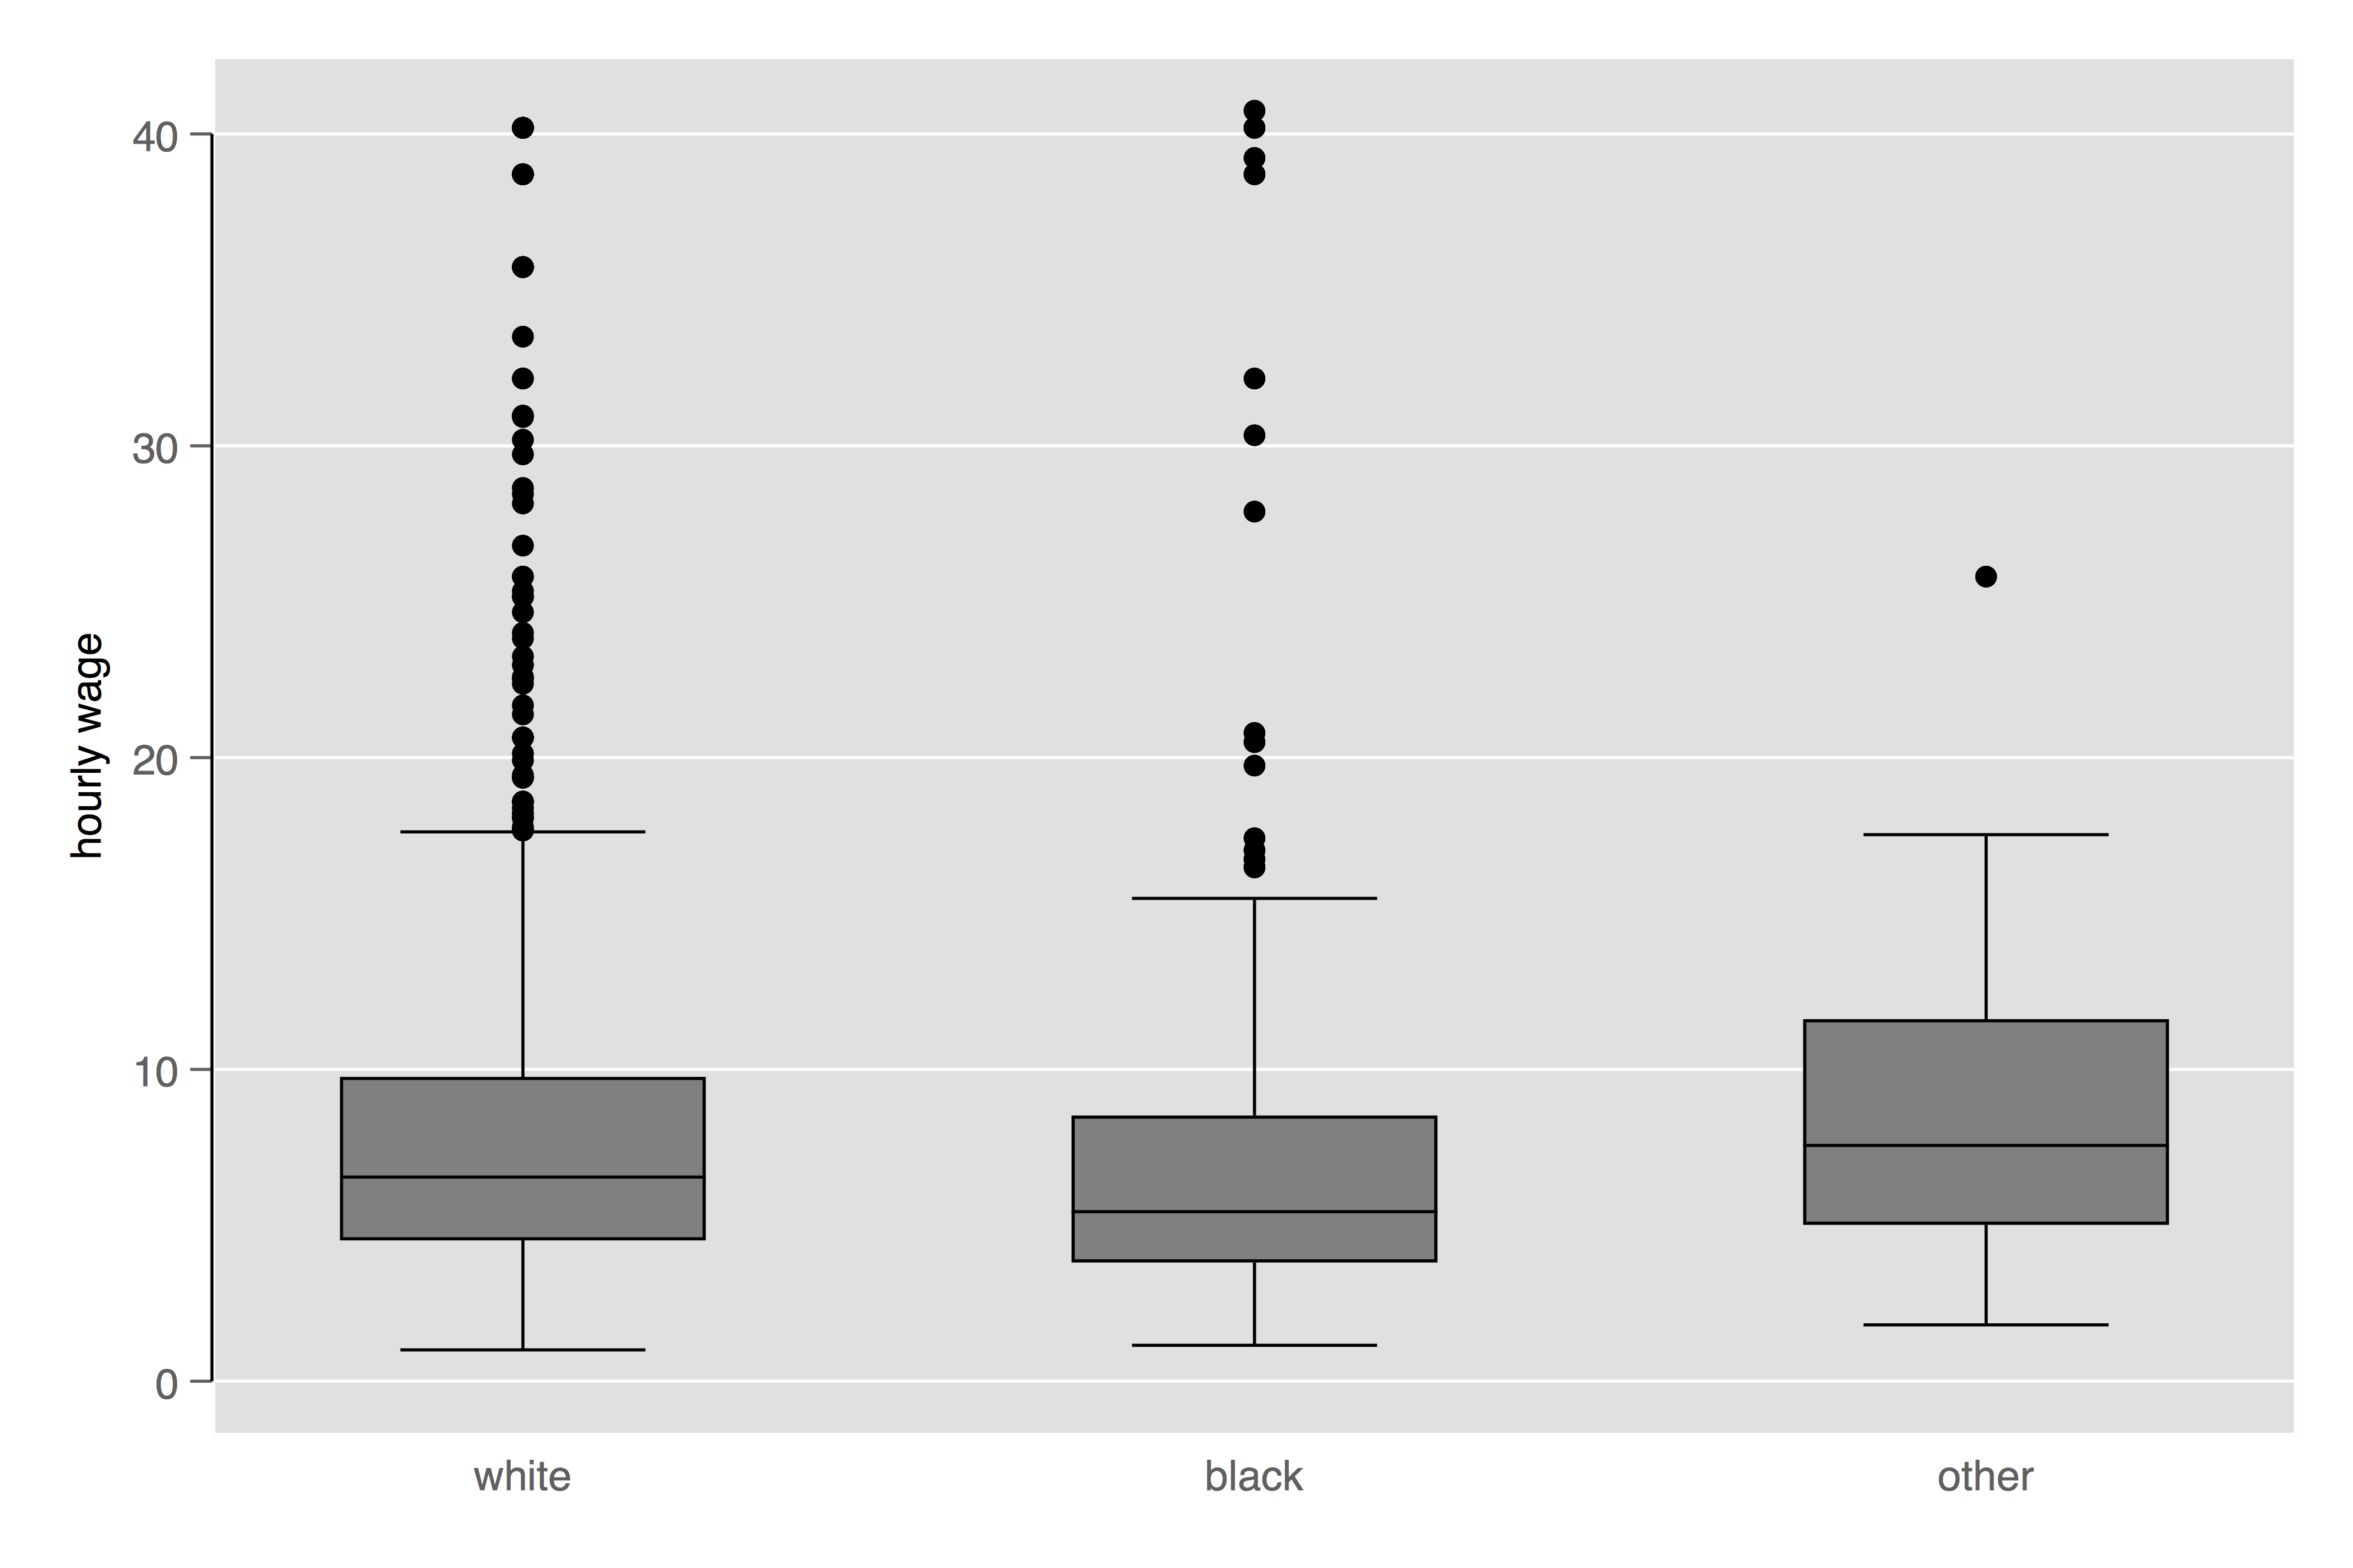
\includegraphics[width=1.00000\textwidth]{race_wage.png}
\caption{}
\end{figure}

What if we wanted to plot these two last scatterplots side-by-side? We
can give each one a name and then combine them:

\begin{stlog}
. scatter weekly_wage grade if race == "black":racelbl, /// 
>    title("Black Women") name(blk_edu_wage, replace) 
{\smallskip}
. scatter weekly_wage grade if race == "white":racelbl, ///
>    title("White Women") name(wht_edu_wage, replace)
{\smallskip}
. graph combine blk_edu_wage wht_edu_wage, ysize(2) xsize(3)
{\smallskip}
. graph export race_edu_wage.png, width(2000) replace
(file race_edu_wage.png written in PNG format)
{\smallskip}
\end{stlog}

\begin{figure}
\centering
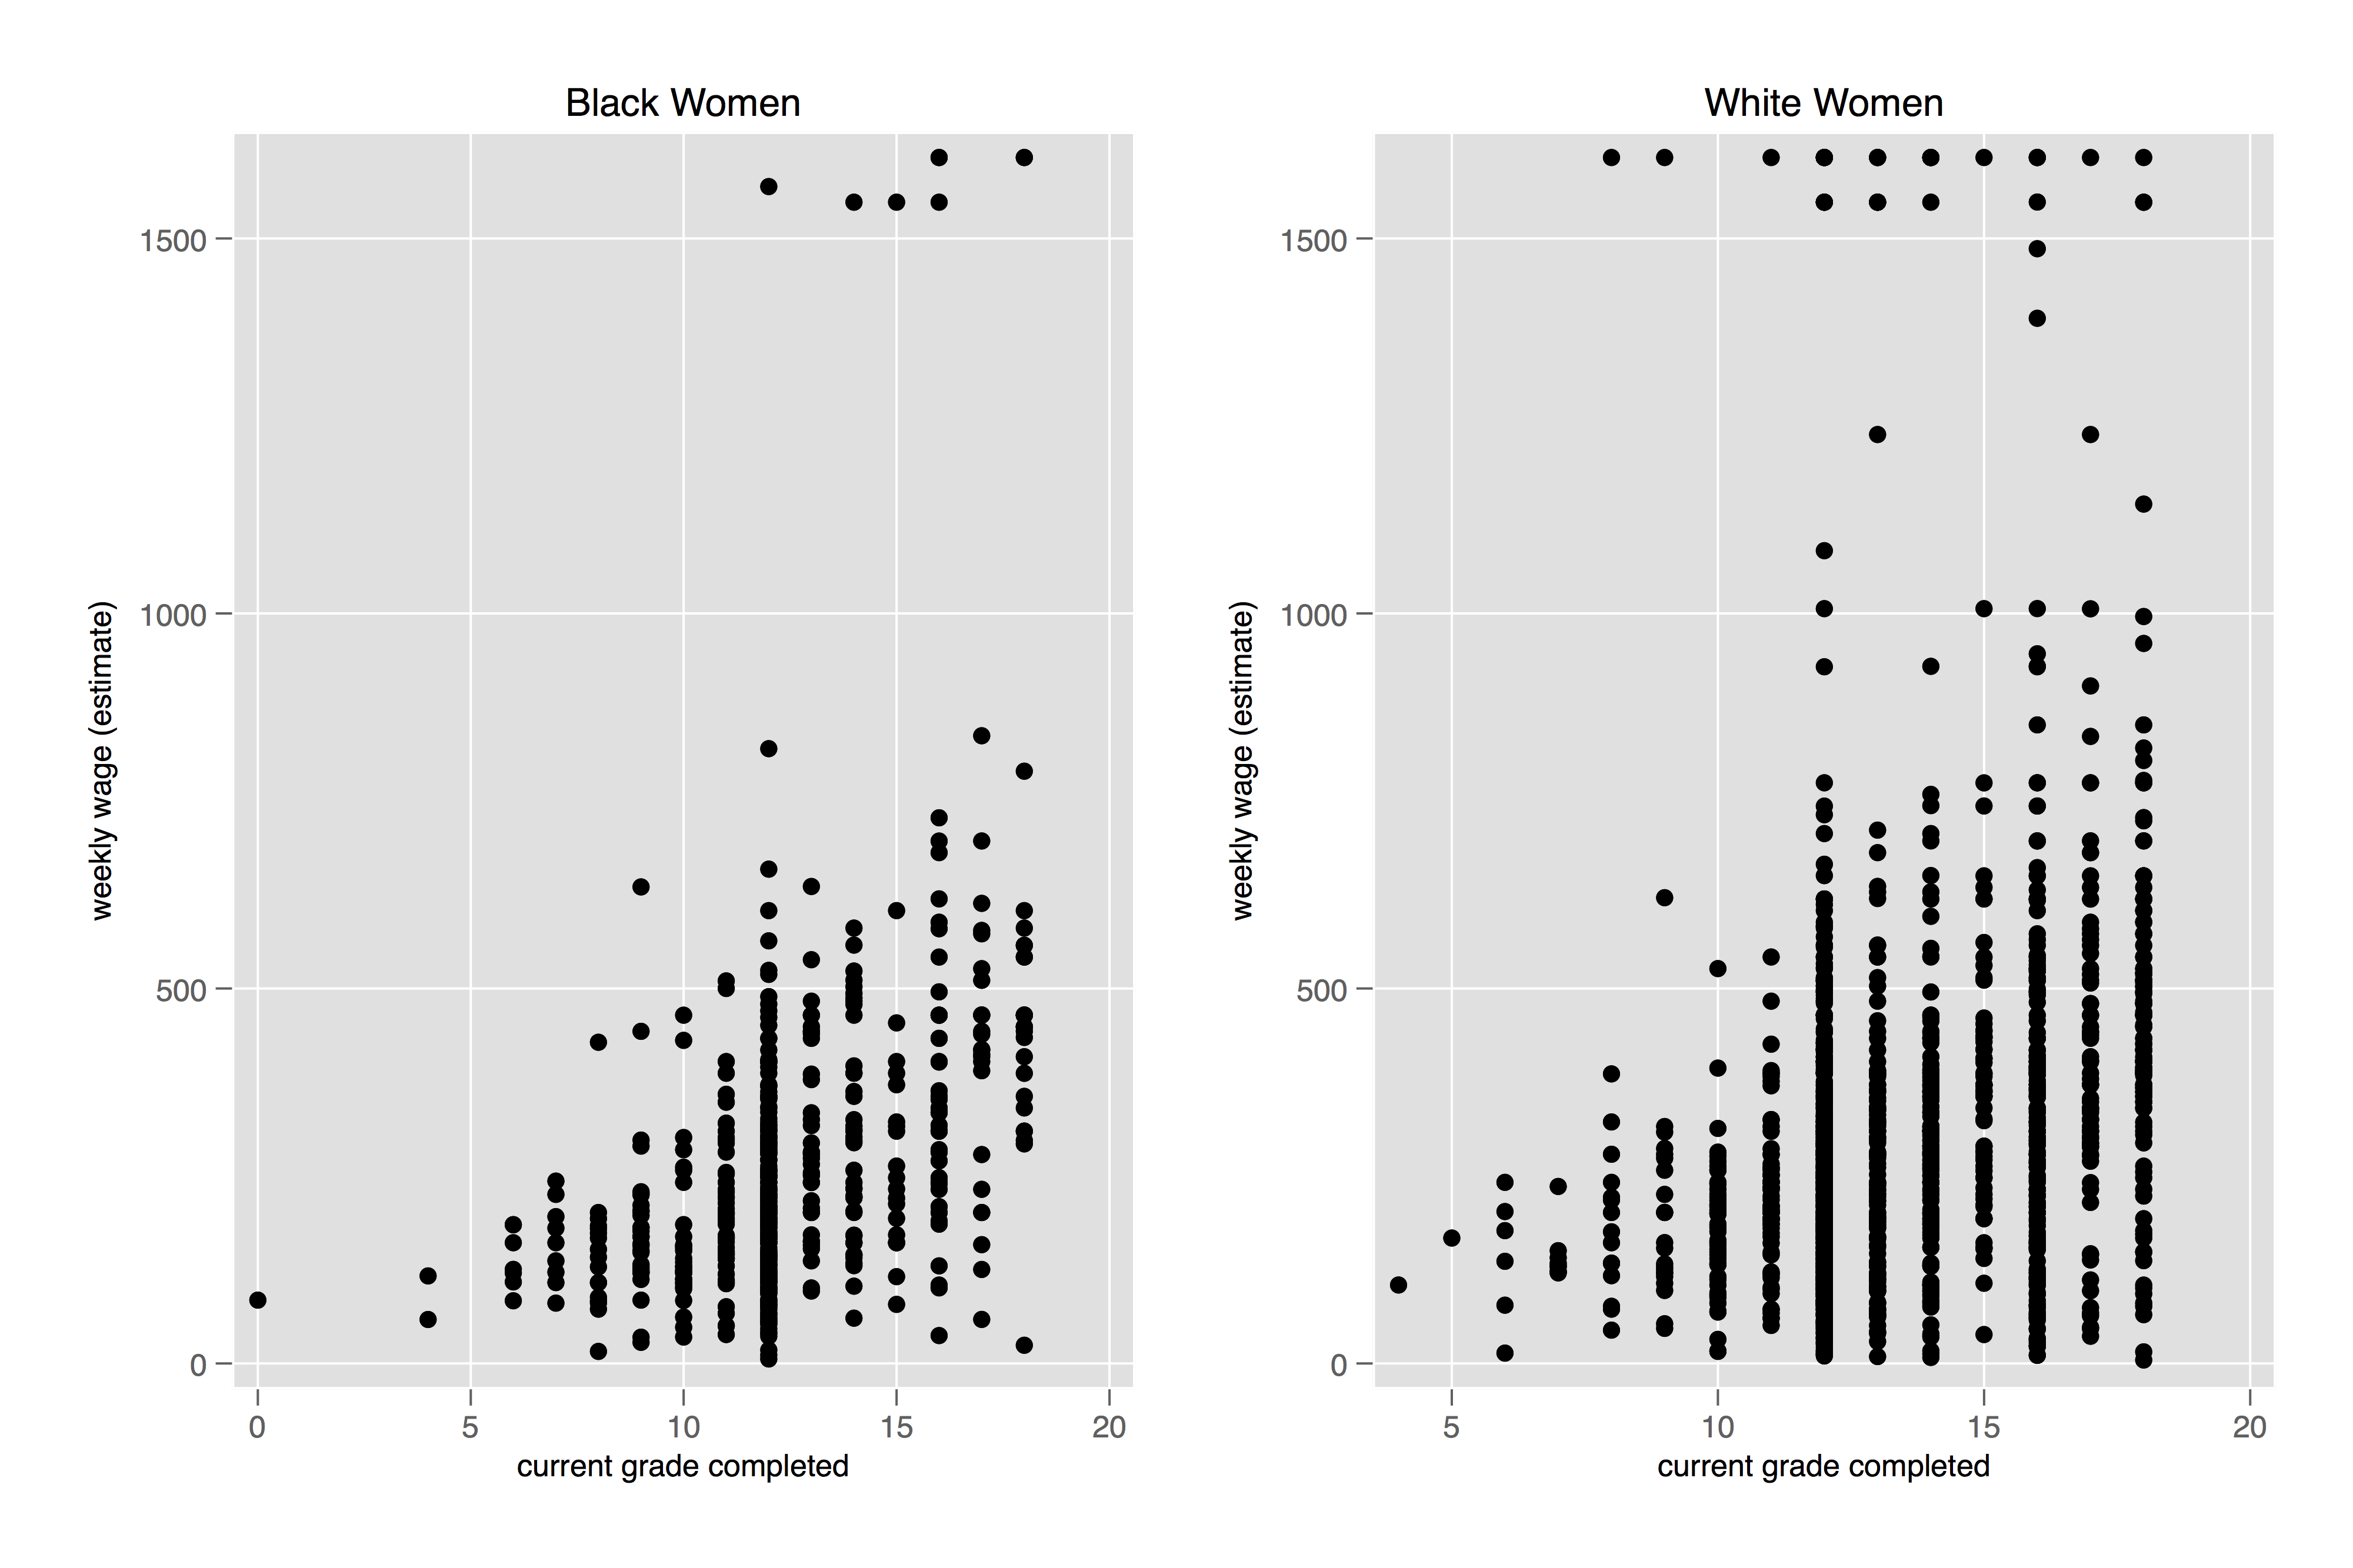
\includegraphics[width=1.00000\textwidth]{race_edu_wage.png}
\caption{}
\end{figure}

\section{A Cheat-sheet for commands}\label{a-cheat-sheet-for-commands}

Unless you are already a Stata flow you will probably need to constantly
refer to online and Stata-based resources on the command names and
syntax of the commands you'd want to run. The Stata manual enclosed in
the Stata Application and online message boards are helpful. A nice
cheat-sheet of commands is here
\url{https://geocenter.github.io/StataTraining/pdf/AllCheatSheets.pdf}

and is also uploaded on Canvas
(https://canvas.harvard.edu/courses/52520/files/folder/Programming-Resources)

\section{More Advanced Topics}\label{more-advanced-topics}

\begin{itemize}
\tightlist
\item
  Writing loops, writing functions, and generating macros are some
  techniques that will greatly simplify -- or will be required -- for
  any work beyond the tabular data provided. We will introduce these
  concepts as necessary, but the tutorial here is a good overview:
  \url{http://data.princeton.edu/stata/programming.html}
\item
  As you deal with multifaceted projects, how you organize your code and
  files will become increasingly important. Better workflow not only
  allows you to work faster, but reduces the number of errors that
  remain uncaught. Gentzkow and Shapiro have a good guide with
  battle-tested tips.
  \url{https://web.stanford.edu/~gentzkow/research/CodeAndData.pdf}
\end{itemize}

\section{Acknowledgements}\label{acknowledgements}

For compilation, I used the \texttt{markstat} package by Germán
Rodríguez. \url{http://data.princeton.edu/stata/markdown}

\end{document}
